\documentclass{article}
\usepackage[spanish]{babel}
\usepackage{amsmath}
\usepackage{amssymb}
\usepackage{lmodern}
\usepackage{xspace}
\usepackage{multicol}
\usepackage{float}
\usepackage{color}
\usepackage{framed}
\usepackage{subfig}
\usepackage{listings}
\usepackage{colortbl}
\usepackage{fancyhdr} 
\usepackage{arxiv}

\usepackage[utf8]{inputenc} % allow utf-8 input
\usepackage[T1]{fontenc}    % use 8-bit T1 fonts
\usepackage{hyperref}       % hyperlinks
\usepackage{url}            % simple URL typesetting
\usepackage{booktabs}       % professional-quality tables
\usepackage{amsfonts}       % blackboard math symbols
\usepackage{nicefrac}       % compact symbols for 1/2, etc.
\usepackage{microtype}      % microtypography
\usepackage{lipsum}		% Can be removed after putting your text content
\usepackage{graphicx}
\usepackage{natbib}
\usepackage{doi}
\usepackage{babel} \usepackage[linesnumbered, ruled, vlined]{algorithm2e}


\newcommand{\X}{\mathbf{X}}
\newcommand{\x}{\mathbf{x}}
\newcommand{\Y}{\mathbf{Y}}
\newcommand{\y}{\mathbf{y}}
\newcommand{\Z}{\mathbf{Z}}
\newcommand{\E}{\mathbf{E}}
\newcommand{\B}{\mathbf{B}}
\newcommand{\w}{\mathbf{w}}
\newcommand{\p}{\mathbf{p}}



\title{Regularización en métodos de regresión}

%\date{September 9, 1985}	% Here you can change the date presented in the paper title
%\date{} 					% Or removing it

\author{ \href{https://orcid.org/0000-0000-0000-0000}{
\includegraphics[scale=0.06]{orcid.pdf}\hspace{1mm}Enrique Santibañez Cortes}\\
	CIMAT\\
	UNIDAD MONTERREY \\
	\texttt{enrique.santibanez@cimat.mx} \\
}

% Uncomment to remove the date
%\date{}

% Uncomment to override  the `A preprint' in the header
%\renewcommand{\headeright}{Technical Report}
\renewcommand{\undertitle}{Presenta:}
%\renewcommand{\shorttitle}{\textit{arXiv} Template}

%%% Add PDF metadata to help others organize their library
%%% Once the PDF is generated, you can check the metadata with
%%% $ pdfinfo template.pdf
\hypersetup{
pdftitle={Regularización en métodos de regresión},
pdfsubject={},
pdfauthor={},
pdfkeywords={Regularización, LASSO, Regresión},
}

\begin{document}
\maketitle

\begin{abstract}
En este trabajo desarrollamos la teoría de los principales métodos de regularización (\textit{Ridge, LASSO y Elastic Net}), enfocándonos en regresión lineal múltiple para poder comprender estos conceptos en su forma más básica. Realizamos una análisis comparativo entre estos métodos, resaltando las ventajas y desventajas que tienen, además de los supuestos que se deben de cumplir para tener buen rendimiento. Posteriormente, realizamos una extensión del método de regularización aplicado en regresión multivariada múltiple presentando la teoría y un ejercicio práctico. Y por último, concluimos resaltando la importancia de estos métodos de regularización que tienen actualmente no solo en problemas de regresión. 
\end{abstract}


\section{Introducción}
Considerando el planteamiento de regresión lineal, 
    \begin{align}\label{regresion}
        y_i = \X\beta+\epsilon,
    \end{align}
donde $\beta, \x_i\in R^p$, y $\X$ es una matriz de tamaño $n\times p$ con renglones $\x_1, \x_2, \cdots, \x_n.$ El método más frecuente para ajustar (\ref{regresion}) es utilizar mínimos cuadrados ordinarios (OLS), el cual consiste en identifica como mejor modelo el hiperplanto que minimiza la suma de errores cuadrados, es decir,
\begin{align}
    \beta^{OLS} =\arg \min_{\beta} \left\{||\y- \X \beta||^2\right\}.
\end{align}
Algunas de las limitaciones que aparecen en la práctica al tratar de emplear este tipo de modelos (ajustados por mínimos cuadrados ordinarios) son:
\begin{itemize}
    \item Se ven perjudicados por la incorporación de predictores correlacionados.
    \item No pueden ajustarse cuando el número de predictores es superior al número de observaciones.
\end{itemize}
En problemas con muchas variables explicativas potenciales que pueden estar en parte altamente correlacionadas entre sí, el enfoque clásico de regresión por mínimos cuadrados puede sufrir el hecho de que los coeficientes de regresión estimados pueden llegar a estar bastante mal determinados, es decir, tener una alta varianza incluso cuando la superficie de regresión ajustada puede estar bien determinada \citep{Boehmke2019HandsOnML}. Entonces, en problemas cuando tenemos $n>p$ y los datos presentan multicolinealidad, una alternativa a la regresión lineal usando mínimos cuadrados es utilizar la regresión regularizada (también conocida como modelos regularizados o métodos de shrinkage) para restringir el tamaño total de todas las estimaciones de coeficientes.

En este trabajo, se describen los fundamentos teóricos y aspectos prácticos de cómo combinar regresión lineal múltiple con métodos de regularización. Las siguientes consideraciones y métodos que aquí se presentan se pueden aplicar tanto para problemas de clasificación como a la regresión en principio. Sin embargo, nos centraremos en modelos de regresión lineal múltiple en la mayor parte de este trabajo.

\section{Métodos de regularización o \textit{shrinkage} en regresión lineal múltiple}

Lo métodos de regularización son estrategias que incorporan penalizaciones en el ajuste por mínimos cuadrados ordinarios con el objetivo de evitar \textit{overfitting}, reducir varianza, atenuar el efecto de la correlación entre predictores y minimizar la influencia en el modelo de los predictores menos relevantes. 

La función objetivo  en un modelo de regresión regularizado es similar al OLS, con un término de regularización $P(\beta)$
\begin{align}
    \arg \min_{\beta} \left\{||\y- \X \beta||^2+P(\beta)\right\}.
\end{align}
Este parámetro de regularización restringe el tamaño de los coeficientes de modo que la única forma en que los coeficientes pueden crecer es si experimentamos una disminución comparable en la suma de errores cuadrados. 

Este concepto se puede generalizar a todos los modelos GLM (ejemplo regresión logística y poisson) e incluso algunos modelos de supervivencias (ver \citep{cox_lasso}). Con la única diferencia en que no necesariamente se deben de tomar la suma de errores cuadrados como función de perdida en los diferentes modelos de GLM o supervivencia. Pero el concepto es el mismo, podemos pensar en el parámetro de regularización que restringe el tamaño de los coeficientes de tal manera que la única forma en que puedan crecer es si experimentamos una disminución comparable en la función de pérdida del modelo.

Tres de los métodos de regularización más empleados son \textit{Ridge, LASSO y Elastic net}. Dado que estos métodos de regularización actúan sobre la magnitud de los coeficientes del modelo, \textbf{todos deben de estar en la misma escala, por esta razón es necesario estandarizar o normalizar los predictores antes de entrenar el modelo} 

\subsection{Ridge}
Cuando hay muchas variables correlacionadas en un modelo de regresión lineal, sus coeficientes pueden estar mal determinados y mostrar una alta varianza. Un coeficiente positivo tremendamente grande en una variable puede ser cancelado por un coeficiente negativo igualmente grande en su primo correlacionado. Los coeficientes de \textit{ridge} minimizan una suma cuadrada del residual penalizada, 
\begin{align} \label{ridge}
\hat{\beta}^{ridge}(\beta) = \arg \min_{\beta} \left\{||\y- \X \beta||^2+\lambda||\beta||_2^2 \right\}
\end{align}
Aquí $\lambda\geq 0$ es un parámetro de complejidad que controla la cantidad de contracción (shrinkage): cuanto mayor es el valor de $\lambda$, mayor es la cantidad de contracción. Los coeficientes se acercan a cero pero no necesariamente son iguales a cero. Una forma equivalente de escribir el problema de \textit{ridge} es
\begin{align}\label{ridge_equi}
    \hat{\beta}^{ridge}(t) &= \arg \min_{\beta} ||\y-\X\beta||_2^2\\
    s.a.&\ \ \  ||\beta||_2^2\leq t,
\end{align}
lo que hace explícita la restricción de tamaño de los parámetros. Existe una correspondencia biunívoca entre los parámetros $\lambda$ en (\ref{ridge}) y $t$ en (\ref{ridge_equi}). Los estimadores de regresión de \textit{ridge} estan dados por 
\begin{align*}
    \hat{\beta}^{ridge} = (\X^T\X+\lambda I)^{-1}\X^T\y
\end{align*}
donde $I$ es una matriz identidad de tamaño $p \times p$. La solución anterior, agrega una constantes positiva a la diagonal $\X^T\X$ antes de calcular la inversa. Esto hace que el problema no sea singular, incluso si $\X^T \X$ no es de rango completo. Esta fue la principal motivación por el cuál se introdujo por primera vez la regresión \textit{ridge} \citep{ridge}.

\subsection{Least absolute shrinkage and selection operator (LASSO)}
LASSO es un método de contracción como \textit{ridge}, con diferencias sutiles pero importantes. La estimación de LASSO se define resolviendo \citep{lasso_original}
\begin{align} \label{lasso_equation}
\hat{\beta}^{lasso}(\beta) = \arg \min_{\beta} \left\{||\y- \X \beta||^2+\lambda||\beta||_1 \right\}
\end{align}
Podemos reescribir el problema anterior como un problema de optimización de la siguiente forma:
\begin{align}\label{lasso_equation_opti}
    \hat{\beta}^{lasso}(t) &= \arg \min_{\beta} ||\y-\X\beta||^2\\
    s.a.&\ \ \  ||\beta||_1\leq t,
\end{align}
Al igual que en \textit{ridge}, el grado de penalización está controlado por $\lambda\geq 0.$ Cuando $\lambda=0,$ el resultado es equivalente estimador por OLS. Y cuando mayor sea $\lambda$, mayor serpa la predicción.\\

Observe el parecido con el problema de regresión utilizando \textit{ridge} (\ref{ridge_equi}) y (\ref{ridge}), la penalización de \textit{ridge} $L_2$ $||\beta||_2$ es remplazada por la penalizacipon $L_1 ||\beta||_1.$ Este cambio hace que las soluciones no sean lineales en $y$, y por lo cuál no existe una expresión de forma cerrada como en el caso de regresión \textit{ridge}, aunque se puede resolver de manera bastante eficiente utilizando algoritmos o métodos como el llamado regresión de ángulo mínimo \citep{lars_efron} o utilizando gradiente descendiente \citep{statisticallearning}. Estos algoritmos tienen el mismo costo computacional que en regresión \textit{ridge}. \citep{statisticallearning}

Debido a la naturaleza de la restricción, hacer $t$ lo suficientemente pequeño hará que algunos de los coeficientes sean exactamente cero, por lo que LASSO hace una especie de selección continua de subconjuntos de variables. 

\subsubsection{Comparación entre Ridge y LASSO}
La principal diferencia práctica entre \textit{LASSO} y \textit{ridge}, es que en \textit{LASSO} es posible obtener coeficientes exactamente iguales a cero. Esto supone una ventaja notable de LASSO en escenarios donde no todos los predictores son importantes para el modelo y se desea que los menos influyentes queden excluidos. En consecuencia, cuando se tiene un problema de regresión con muchos predictores, LASSO se puede utilizar paraa identificar y extraer aquellas características \textit{más importantes}.
\begin{figure}[H]
\centering
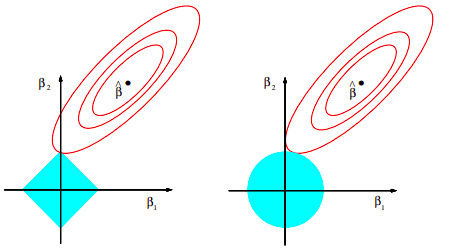
\includegraphics[scale=0.5]{figure/comparacion_regiones.png}
\caption{Regiones de los problemas de optimización, \citep{statisticallearning}}
\end{figure}
Por otro lado, cuando existen predictores altamente correlacionados (linealmente), \textit{ridge} reduce la influencia de todos ellos a la vez y de forma proporcional, mientras que LASSO tiende a seleccionar uno de ellos, dándole todo el peso y excluyendo al resto. En presencia de correlaciones, esta selección varía mucho con pequeñas perturbaciones (cambios en los datos de entrenamiento), por lo que, las soluciones de LASSO, son muy inestables si los predictores están altamente correlacionados. Por lo que en estos casos es recomendable utilizar regularización \textit{ridge.}

Para conseguir un equilibrio óptimo entre estas dos propiedades (multicolinealidad y subgrupo de variables relevantes), se puede emplear lo que se conoce como penalización elastic net, que combina ambas estrategias.

\subsection{Extensión LASSO}
\cite{statisticallearning} mencionan que la regularización $L1$ de LASSO a tenido mucha relevancia, hasta el punto de desarrollar la detección de un campo comprimido en la literatura sobre procesamiento de señales. En esta subsección mencionaremos algunas de ellas, sin entrar mucho a detalle.
\subsubsection{Elastic net}
\cite{elastic_net} presentan por primera vez este enfoque de penalización, el cual es una generalización de las penalización \textit{ridge} y \textit{LASSO}, llamado \textit{elastic net}. La estimación de \textit{elastic net} se define 
\begin{align}\label{elastic_net_equation}
    \hat{\beta} = \arg \min_{\beta} \{||\y-\X \beta ||^2+\lambda_2||\beta||^2+\lambda_1||\beta||\}
\end{align}
Sea $\alpha = \lambda_2/(\lambda_1+\lambda2),$ entonces resolver $\hat{\beta}$ en (\ref{elastic_net_equation}) es equivalente a el siguiente problema de optimización
\begin{align}
    \hat{\beta} &= \arg \min_{\beta} \left\{ ||\y-\X\beta||^2 \right\}\\
    s.a. &\ \ \ (1-\alpha)||\beta||+\alpha||\beta||^2\leq t.
\end{align}

Aunque los modelos de \textit{LASSO} realizan la selección de características, cuando dos características fuertemente correlacionadas se empujan hacia cero, una se puede empujar completamente a cero mientras que la otra permanece en el modelo. Además, el proceso de uno dentro y otro fuera no es muy sistemático. Por el contrario, la penalización por regresión de la cresta es un poco más eficaz en el manejo sistemático de características correlacionadas juntas. En consecuencia, la ventaja de la penalización de la \textit{elastic net} es que permite una regularización eficaz a través de la penalización de \textit{ridge} con las características de selección de características de la penalización del \textit{LASSO}.

\subsubsection{LASSO adaptativo}
\cite{lasso_adaptative} presenta una condición necesaria para que la selección de la variable \textit{LASSO} sea consistente. En consecuencia, existen ciertos escenarios donde el \textit{LASSO} es inconsistente para la selección de variables. Proponen una nueva versión del LASSO, llamado \textit{LASSO} adaptativo. La función a optimizar en este caso es
\begin{align} \label{lasso_adaptatico_equation}
\hat{\beta}^{lasso_ada}(\beta) = \arg \min_{\beta} \left\{||\y- \X \beta||^2+\w\lambda||\beta||_1 \right\}
\end{align}
donde $\w$ es un vector de pesos conocidos. Se puede mostrar que el \textit{LASSO} adaptativo disfruta de las propiedades del oráculo, es decir, funciona tan bien como si el verdadero modelo subyacente se diera de antemano. Además, el \textit{LASSO} adaptativo se puede resolver con el mismo algoritmo eficiente para resolver el \textit{LASSO}.

\subsubsection{LASSO grupal}
Cuando existe de variables predictores que pertenecen a grupos definidos, por ejemplo una colección de variables indicadores para representar los niveles de un predictor categórico. En estas situación, \cite{statisticallearning} menciona que es conveniente reducir y seleccionar a los miembro de un grupo juntos, lo cual es el concepto principal de \textit{LASSO} agrupado.

Suponga que los $p$ predictores se dividen en $L$ grupos con $p_l$ el número del grupo $l$. Para facilitar la notación, usamos una matriz $X_l$ para representar los predictores correspondientes en el $l-$ésimo grupo, con el vector de coeficientes correspondiente $\beta_l.$ Entonces la función a minimiza con este plantamento es
\begin{align}
    \hat{\beta}^{lasso_grupo}(\beta) = \arg \min_{\beta} \left\{||\y- \X \beta||^2+\sqrt{\p}\lambda||\beta||_2 \right\}
\end{align}
donde $\sqrt{p}=\begin{pmatrix}p_1& \cdots & p_l \end{pmatrix}$ son los diferentes tamaños de los grupos.
\section{Resultados numéricos}
Para comparar los efectos entre los distintos métodos de regularización y el efecto del parámetro de regularización, realizamos dos problemas de regresión lineal múltiple en dónde existen evidencia de multicolinealidad en donde el enfoque de mínimos cuadrados no tiene buen rendimiento.

\subsection{Ejemplo: Datos de delitos (diferencias de los métodos de regularización y el parámetro de regularización)}
El objetivo de este análisis es poder predecir el el número de crímenes violentos a partir de un conjunto de aspectos poblacionales: porcentaje de la población considerada urbana y el ingreso familiar medio, y la participación de las fuerzas del orden público, como el número per cápita de agentes de policía y el porcentaje de agentes asignados a las unidades de drogas, etc. Estos datos fueron obtenidos del repositorio de Aprendizaje Automático de UCI \citep{datos_uic}. Se tiene 122 variables explicativas y una variable respuesta crímenes violentos, los cuales están normalizaron en el rango decimal $0.00-1.00$ \citep{linear_regression_with_r}. 

Las correlación de estas variables es alta (ver Figura \ref{fig:matriz_cor_ejer1}), lo que supone un problema a la hora de emplear modelos de regresión lineal. Por lo que incita a utilizar una alternativa de regularización. Para medir el impacto de la regularización primero implementamos la estimación por OLS como y \textit{baseline} de este ejercicio, utilizando como métrica el error cuadrático medio (RMSE). 
\begin{figure}[H]
    \centering
    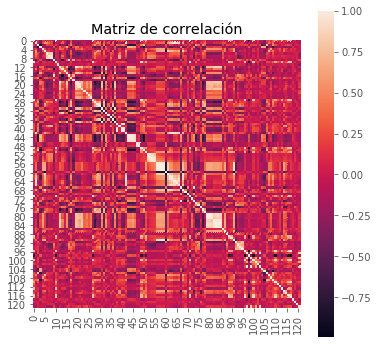
\includegraphics[scale=0.4]{figure/matriz_cor_ejer1.png}
    \caption{Heatmap de la matriz de correlación entre las 122 variables predictoras.}
    \label{fig:matriz_cor_ejer1}
\end{figure}
Para este ejercicio utilizamos un conjunto de prueba y de entrenamiento. El modelo de regresión por OLS arroja un RMSE de 0.3097 en el conjunto de prueba. Posteriormente ajustamos modelos de regresión con regularización de \textit{ridge}, \textit{LASSO} y \textit{elastic net}, y para determinar el mejor valor de $\lambda$ utilizamos validación cruzada utilizando 10 folds, los valores probados fueron considerando los números 200 espaciados uniformemente en una escala logarítmica entre -4 y 1. 

Podemos notar claramente, que cuando se utilizan la regularización \textit{ridge} que entre más grande sea el valor de $\lambda$ hace que los coeficientes se acerquen a cero, pero no necesariamente sean cero. Que a diferencia con la regularización $LASSO$ vemos que entre más grande sea $\lambda$ de igual manera los coeficientes se van acercando a cero hasta llegar a cero. 
\begin{figure}[H]
    \centering
    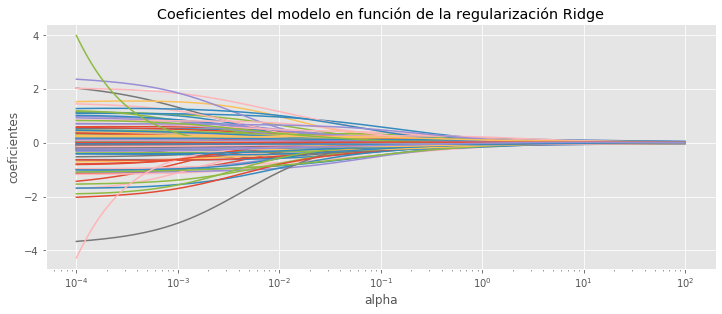
\includegraphics[scale=0.3]{figure/coef_ridge_ejer1.png}
    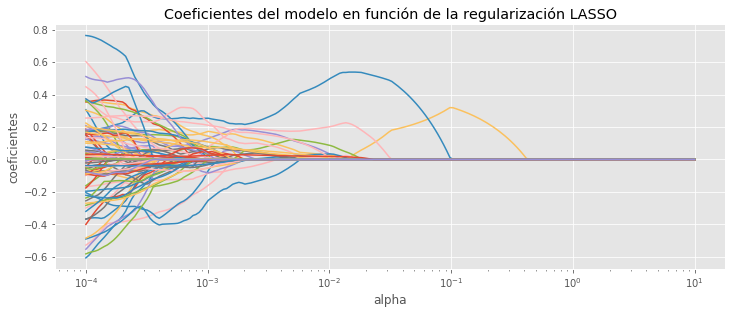
\includegraphics[scale=0.3]{figure/coef_lasso_ejer1.png}
    \caption{Comparación de los coeficientes entre rigde y \textit{LASSO} utilizando diferentes valores de $\lambda$}
    \label{fig:coef_lasso_ejer1}
\end{figure}

Posteriormente utilizando los mejores valores de $\lambda$ obtenidos por validación cruzada para cada uno de las regularizaciones calculamos el RMSE en el conjunto de prueba (ver Figura \ref{fig:comparacion_errores_ejer1}). Podemos notar que los tres métodos de regularización tienen mejores RMSE en comparación con el ajuste de OLS, estos resultados tienen sentido debido a que los datos tenías multicolinealidad. 
\begin{figure}[H]
    \centering
    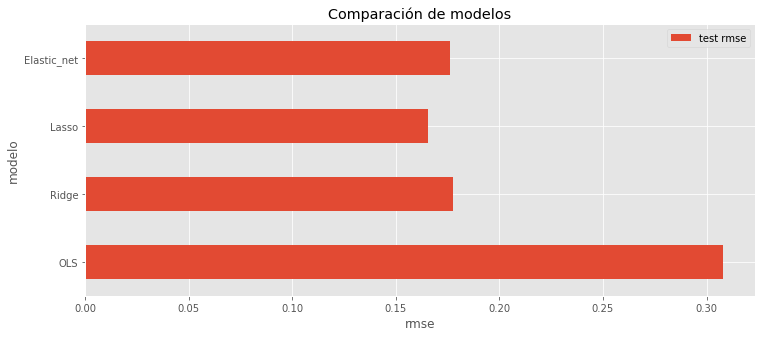
\includegraphics[scale=0.4]{figure/comparacion_errores_ejer1.png}
    \caption{Comparación del RMSE para los distintos ajustes}
    \label{fig:comparacion_errores_ejer1}
\end{figure}
El mejor modelo fue utilizando regularización \textit{LASSO}, una gran diferencias con los dos métodos de regularización es que este método considera solamente 22 variables predictoras y el resto de los coeficientes son valores iguales a 0 (ver Figura \ref{fig:coef_lasso_ejer1}). De igual manera, vemos que cuando $\lambda$ crece esto implica que el número de coeficientes iguales a cero aumenta. 
\begin{figure}[H]
    \centering
    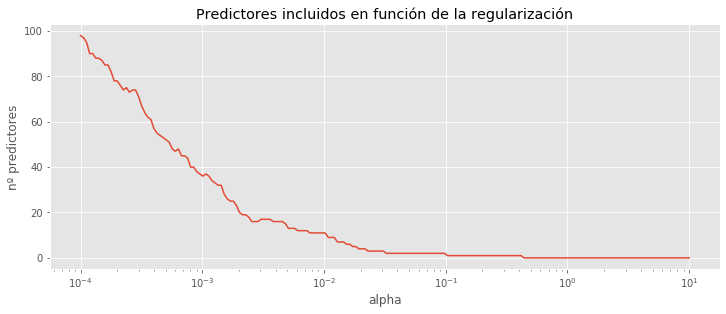
\includegraphics[scale=0.3]{figure/cero_lasso_ejer1.png}
    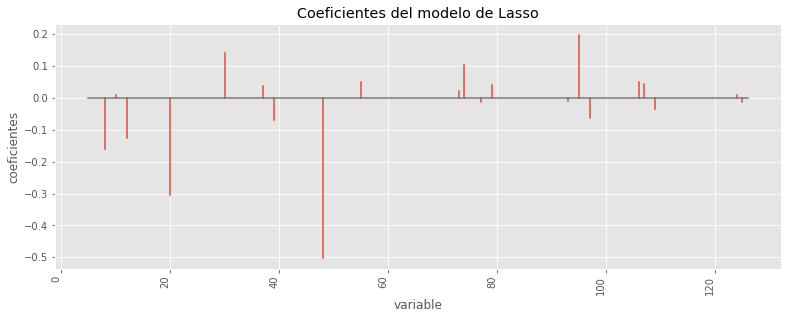
\includegraphics[scale=0.3]{figure/lasso_ejer1.png}
    \caption{Número de coeficientes diferentes de cero y coeficientes de la mejor configuración en \textit{LASSO}}
    \label{fig:coef_lasso_ejer1}
\end{figure}
Este resultado es muy importante cuando se desea considerar el comportamiento de los datos a analizar. Es decir, considerando que en regresión hay dos objetivos en un análisis (predictor y descriptivo), en ocasiones es preferible modelos en donde se tenga menos variables debido a que esto tiene más interpretación que modelos que tienen más variables. Obviamente esta ganancia en la interpretación esta relacionada con el aumente en el error de predicción. 

\subsection{Ejemplo: Contenido de grasa (efecto de escalas)}
Este ejercicio y los datos fue propuesto por \cite{Boehmke2019HandsOnML}, con una pequeña modificación para observar el impacto de estandarizar los datos en los métodos de regularización. Se tiene un departamento de calidad de una empresa de alimentación se encarga de medir el contenido en grasa de la carne que comercializa. Este estudio se realiza mediante técnicas de analítica química, un proceso relativamente costoso en tiempo y recursos. Una alternativa que permitiría reducir costes y optimizar tiempo es emplear un espectrofotómetro (instrumento capaz de detectar la absorbancia que tiene un material a diferentes tipos de luz en función de sus características) e inferir el contenido en grasa a partir de sus medidas.

Antes de dar por válida esta nueva técnica, la empresa necesita comprobar qué margen de error tiene respecto al análisis químico. Para ello, se mide el espectro de absorbancia a 100 longitudes de onda (variables predictoras) en 215 muestras de carne (número de registros), cuyo contenido en grasa se obtiene también por análisis químico. Entonces el objetivo es predecir el contenido en grasa a partir de los valores dados por el espectrofotómetro.

Entonces para medir el efecto que tiene estandarizar los datos en los métodos de regularización, multiplicamos los datos de los últimas 20 variables predictoras por un factor de expansión de 10000. Posteriormente, veamos que la matriz de correlación de nuestras diferentes longitudes de ondas (ver Figura \ref{fig:matriz_cor_ejer2}) presenta un efecto muy fuerte de multicolinealidad, por lo que en teoría el método de regularización se espera que tenga mejores resultados con los otros métodos de regularización.  
\begin{figure}[H]
    \centering
    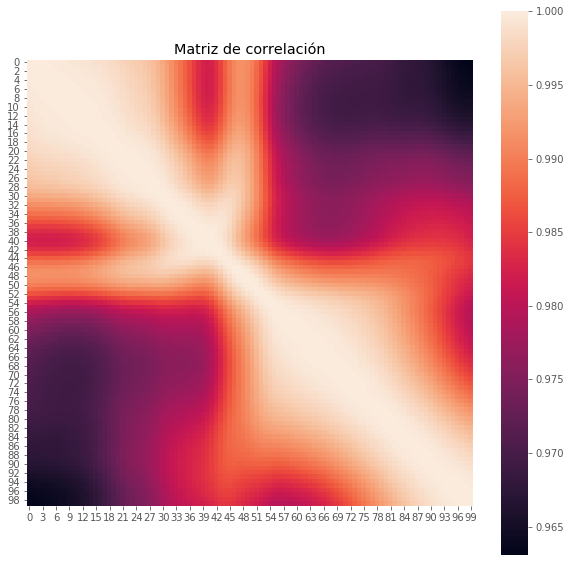
\includegraphics[scale=0.3]{figure/matriz_cor_ejer2.png}
    \caption{Heapmap de la matriz de correlación de nuestras longitudes de onda}
    \label{fig:matriz_cor_ejer2}
\end{figure}
Utilizamsos validación cruzada para obtener el mejor valor de $\lambda$ de los métodos de regularización con los datos originales y a los datos estandarizados. Posteriormente, calculamos el RMSE en nuestro conjunto de prueba (ver Figura \ref{fig:comparacion_errores_ejer2}). Se observa claramente que el efecto de ajustar los métodos de regularización de los datos originales y datos estandarizados. Además, se observa que la regularización \textit{ridge} presenta los mejores resultados. 
\begin{figure}[H]
    \centering
    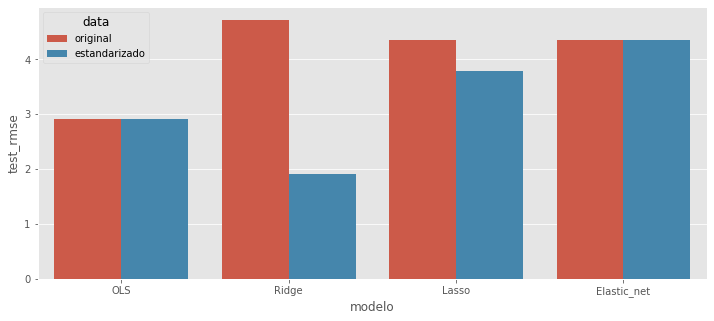
\includegraphics[scale=0.4]{figure/comparacion_errores_ejer2.png}
    \caption{Comparación del RMSE  en estandarizados y originales.}
    \label{fig:comparacion_errores_ejer2}
\end{figure}
Este resultado demuestra la importancia de utilizar los datos estandarizados, este supuesto debe de ser considerado a la hora de considerara métodos de regularización.


\section{Extensión de regularización para el caso multivariado}
\label{multivariado}
En esta sección tienen el objetivo de extender el método de regularización para el caso de regresión lineal multivariada, con el fin de ver la facilidad de implementación en otros modelos distintos a la regresión lineal. Además se presenta un ejemplo numérico en donde se observa la importancia que tiene los métodos de regularización en contra del enfoque clásico. 

\subsection{Regresión lineal multivariada.}
La regresión multivariada es una generalización del modelo de regresión clásico pero considerando $q>1$ variables respuestas. Es decir, sea $\X$ la matriz de las variables independientes $n\times p$, $\Y$ la matriz de las variables independientes $n\times q$ y sea $\E$ la matriz de error aleatorio $n\times q$. Entonces el modelo de regresión multivariada es
\begin{align}
        \Y = \X \B +\E,
\end{align}
donde $\B$ es la matriz de coeficientes de regresión $p\times q$. Si $q=1$ el modelo se simplifica al problema de regresión clásico donde $\B$ es el vector de coeficientes de regresión $p-$dimensional. Consideremos que las $\X$ y $\Y$ están centradas para facilitar los cálculos.\\

La función de verosimilitud logarítmica negativa de ($\B, \Omega$), donde $\Omega = \Sigma^{-1}$ se puede expresar como 
\begin{align} \label{log_verosimilitud}
    g(\B,\Omega) = \tr \left[ \frac{1}{n}(\Y-\X\B)^T(\Y-\X\B)\Omega \right] -\log(\det(\Omega))
\end{align}
Es fácil ver (derivando con respecto a $\B$ e igualando a 0, y simplificando), que el estimador de máxima verosimilitud de $\B$ es 
\begin{align} \label{estimador_B_OLS}
    \hat{\B}^{OLS}=(\X^T\X)^{-1}\X^T\Y.
\end{align}
Lo anterior es equivalente a realizar las estimaciones de $\B$ utilizando mínimos cuadrados ordinarios de forma separada para cada una de las q variables de respuestas y no este implica que no dependan  de $\Omega.$ 

\subsection{Estimación}
De lo anterior podemos observar dos enfoques distintos cuando se considera una regresión multivariada. Lo primero es considerar que los datos no están correlacionados, es decir, que no dependan de $\Omega$ y el otro enfoque es considerar la matriz de covarianzas de los errores. Pero en ambos métodos agregamos un parámetro de regularización.

\subsubsection{Regularized  Multivariate regression for identifying Master Predictors (REMMAP)}

El problema de minimización con restricciones propuesto por \citep{remap}, considera una optimización L1 y L2, considera tambien que las q respuestas observadas no estan correlacionadas,  la función a optimizar es representada como:
\begin{align*}
&L(\hat{\B},\X,\Y)=  \underset{B}{argmin} \{ ||(\Y-\X\B)'(\Y-\X\B)||^{2}  + \lambda_1 \sum_{j} \sum_{k} |b_{jk}|  + \lambda_2 \sum_{j} \sum_{k} (b_{jk})^{2} \} 
\\ &L(\hat{\B},\X,\Y)=  \underset{\B}{argmin}  \{\frac{1}{2} \sum_{k=1}^{q} (\y_{k}-\x \B_{k})^{2} \} + \lambda_1 \sum_{k=1}^{q}|\B_{k}| +  \lambda_2 \sqrt{\sum_{k=1}^{q}(\B_{k})^{2}}  \}
\end{align*}  
Considerando $\lambda_2=0$, pues solo trabajaremos con la restricción de norma L1, tenemos:
$$ L(\hat{\B},\X,\Y)=  \underset{\B}{argmin} \{\frac{1}{2} \sum_{k=1}^{q} (\y_{k}-\x \B_{k})^{2} \} + \lambda_1 \sum_{k=1}^{q}|\B_{k}| $$

La metodología de regresión \textit{LASSO} y la búsqueda del resultado utilizando un algoritmo de descenso coordinado, fue tratado para el caso de la regresión múltiple específicamente en \citep{mrce}, donde la actualización de la función se realiza de manera idéntica considerando una única variable respuesta k, además observemos que dado que los datos están estandarizados la norma del vector seria igual a n, es decir $||\X_{j_0}||^{2}_2=n$. De esto ultimo observamos que el resultado de aplicar el algoritmo seria k regresiones \textit{LASSO} (ver \textbf{Algoritmo \ref{REMMAP_al}}).

\subsubsection{Regresión multivariada con estimación de covarianza (MRCE)}
\cite{mrce} plantea un procedimiento para construir un estimador de una matriz de coeficientes de regresión multivariada que tenga en cuenta la correlación de las variables de respuesta. Básicamente propone un estimador para $\B$ que considera los errores correlacionados utilizando la verosimilitud normal. Considera dos penalizaciones a la verosimilitud logarítmica negativa (\ref{log_verosimilitud}) para construir un estimador disperso $\B$ que dependa de $\Omega=\{\omega_{j'j}\}$,
\begin{align}\label{log_verosimilitu_penalizado}
    (\hat{\B}, \hat{\Omega}) = \arg \min_{\B, \Omega} \left\{g(\B, \Omega)+\lambda_1\sum_{j'\neq j} |\omega_{j'j}| +\lambda_2\sum_{j=1}^p\sum_{k=1}^q|b_{jk}|\right\} 
\end{align}
donde $\lambda_1\geq 0$ y $\lambda_2\geq 0$ son los parámetros de regularización. Se considera una penalización del \textit{LASSO} en las entradas fuera de la diagonal de la covarianza del error inverso $\Omega$ por dos razones.
\begin{enumerate}
    \item Se asegura una solución óptima para $\Omega$ tenga un valor finito cuando hay más respuestas que muestras ($q>n$).
    \item Tiene un efecto de reducir el número de parámetros en la covarianza del error inverso, lo cuál es útil cuando $q$ es grande. \citep{Rothman_2008}.
\end{enumerate}
Y la penalización \textit{LASSO} en $\B$ introduce escases en $\hat{\B}$, que reduce el número de parámetros en el modelo y proporciona una interpretación a los coeficientes. Además, esta penalización implica una solución óptima para $\B$ en función de $\Omega$. Cabe resaltar, que sin una penalización en $\B$ (es decir, $\lambda_2=0$) la solución óptima para $\B$ es siempre $\hat{\B}^{OLS}$ [\ref{estimador_B_OLS}].\\

El problema de optimización en (\ref{log_verosimilitu_penalizado}) no es convexo, sin embargo, resolver $\B$ o $\Omega$ con el otro parámetro fijo hace al problema convexo. Entonces, si dejamos fijo $\B$ en un punto $\B_0$ el problema de optimización para $\Omega$ se convierte a 
\begin{align} \label{cov_estimate}
    \hat{\Omega}(\B_0) = \arg \min \left\{ tr \left(\hat{\Sigma}_R \Omega \right)-\log(\det\Omega) +\lambda_1\sum_{j'\neq j}|\omega_{j'j}|)\right\},
\end{align}
donde $\hat{\Sigma}_R=\frac{1}{n}(\Y-\X\B_0)^T(\Y-\X\B_0).$ Este problema es conocido como el problema de estimación de covarianza considerando una penalización $L_1$. \cite{friedman_sparse_2008} plantea el algoritmo de \textit{LASSO} gráfico para resolver el problema de optimización \ref{cov_estimate}. Se abordará con más detalle este algoritmo en las secciones posteriores.

Por otro lado, resolver \ref{log_verosimilitu_penalizado} fijando $\Omega$ en un punto elegido $\Omega_0$ transforma el problema a optimizar
\begin{align}\label{est_beta}
    \hat{\B}(\Omega_0) = \arg \min \left\{ tr \left( \frac{1}{n}(\Y-\X\B)^T(\Y-\X\B)\Omega_0+\lambda_2 \sum_{j=1}^p\sum_{k=1}^q |b_{jk}| \right) \right\}
\end{align}
Una solución para el problema anterior es utilizar un descenso de coordenadas cíclicas. \cite{mrce} resume en el procedimiento de optimización como se describe en el \textbf{Algoritmo \ref{algoritmo_1}} (ver Anexos). Se utiliza la estimación de mínimos cuadrados penalizados por rigde $\hat{\B}^{ridge}=(\X^T\X+\lambda_2I)^{-1}\X^T\Y$ para escalar nuestra prueba de convergencia de párametroas, ya que siempre está bien definida (incluso cuando $p>n$). La derivación completa del algoritmo se puede ver en la \textbf{Sección \ref{descenso_coo}}.

Considerando lo anterior, podemos resumir la resolución del problema de optimización (\ref{log_verosimilitu_penalizado}) usando el descenso de coordenadas en bloque, es decir, iteramos minimizando con respecto a $\B$ y minimizando con respecto a $\Omega$. El \textbf{Algoritmo \ref{algoritmo_2}} (ver Anexos) usa el descenso de coordenadas por bloques para calcular una solución loca para (\ref{log_verosimilitu_penalizado}). 

\subsection{Ejemplos: Datos sintéticos (efecto $n>p$)}
Recordando que los estimadores de OLS tienen problemas cuando existen un número mayor de predictores que de observaciones, entonces para verificar este hecho lo probamos en esta extensión de regularización. 
\subsection{Evaluación de los modelos con datos sintéticos}
El conjunto de datos sintéticos fue generado con la función $make_regression()$ de la librería de Scikit-learn \citep{scikit-learn}. Consideramos diferentes parámetros de la función anterior: $n\_samples (n)=[100,20],\  n\_features(p)=[20,100],$ y $ n\_targets(q)=[2,5]$. Esto con el objetivo de observar el efecto que tiene las dimensiones de diferentes datos en nuestros modelos. Consideramos partir el conjunto de datos original, en dos conjuntos uno de prueba y otro de entrenamiento. Además de que nuestro conjunto de datos, consideramos una estandarización debido a los supuestos que se tienen en los modelos.

Para el caso en el que $n>p$, los rendimientos de regularización no son buenos en comparación con el enfoque clásico de OLS (ver Figura \ref{R}). Esto tiene completamente sentido debido a que nuestros datos sintéticos son creados sin considerar correlaciones entres las variables y por lo tanto no existe ninguna incumplimiento en los supuestos de OLS. Además, vemos que MRCE es muy parecido a OLS esto debido a la relación que existe cuando $\lambda =0.$ 
\begin{figure}[H]
 \minipage{0.5\textwidth}
   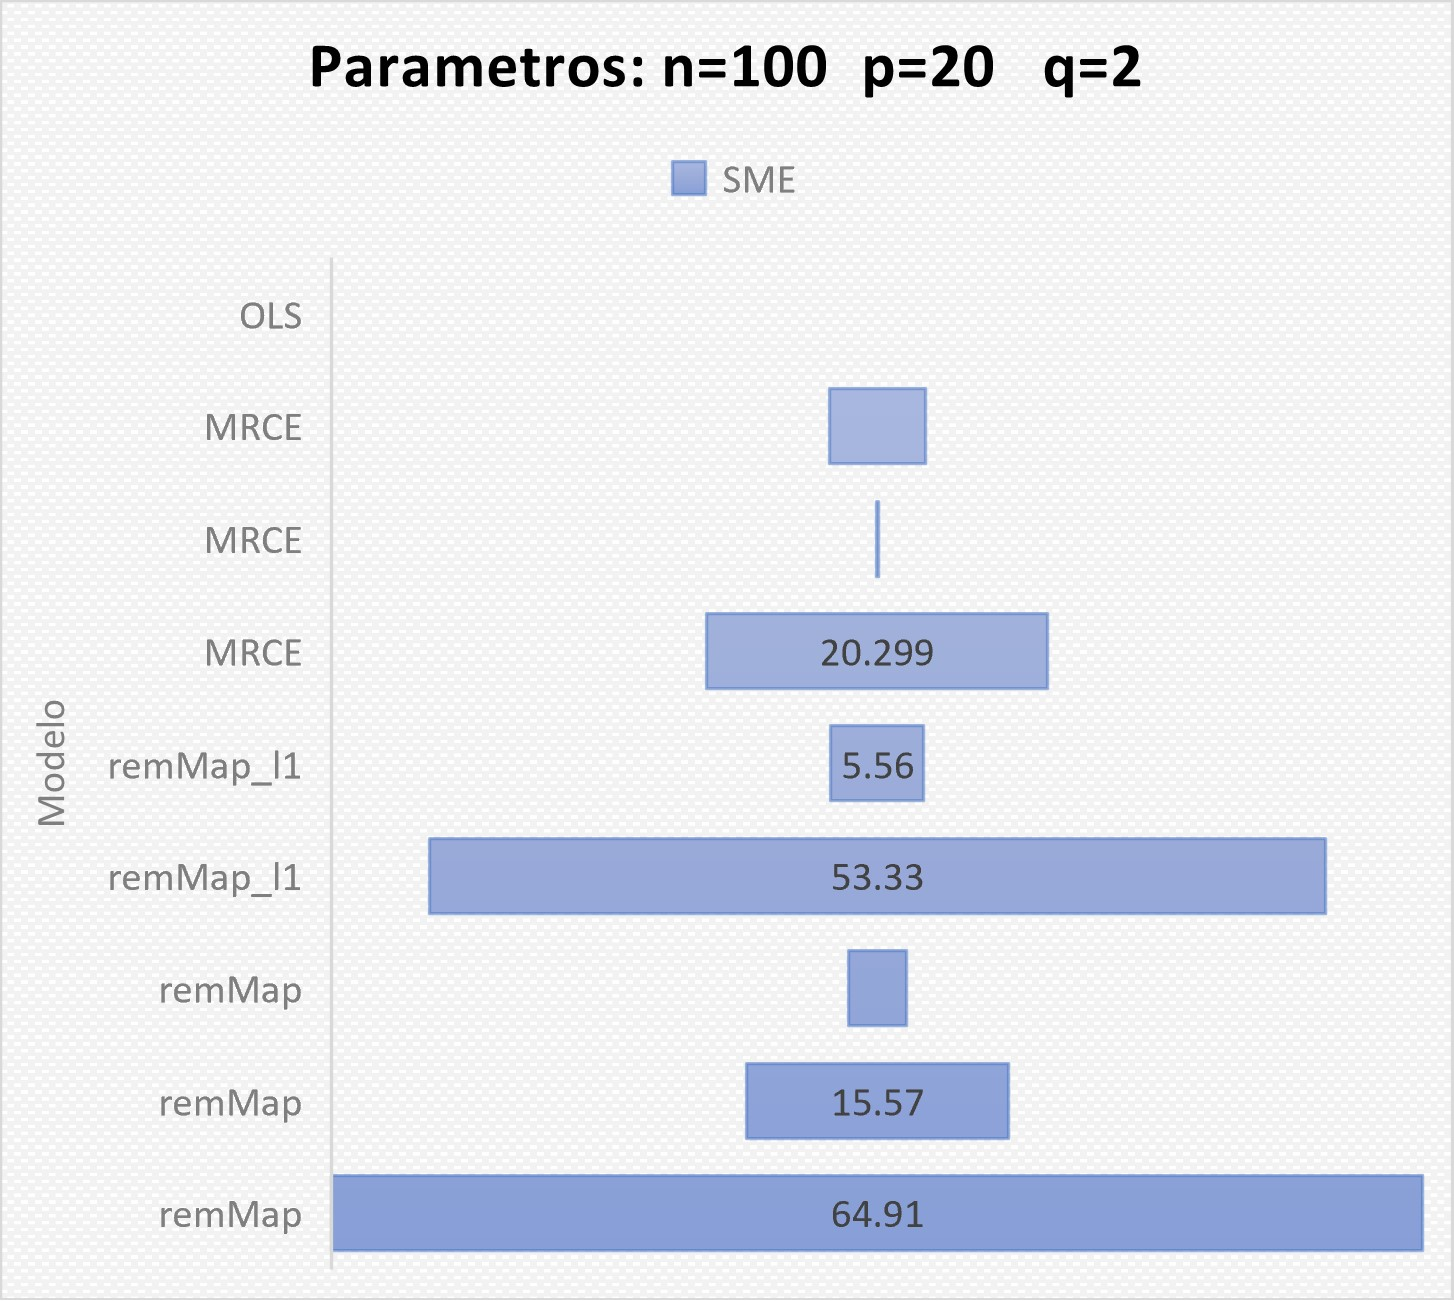
\includegraphics[scale=.65]{figure/im3.jpg}
  \caption{}
 \endminipage
 \minipage{0.5\textwidth}
   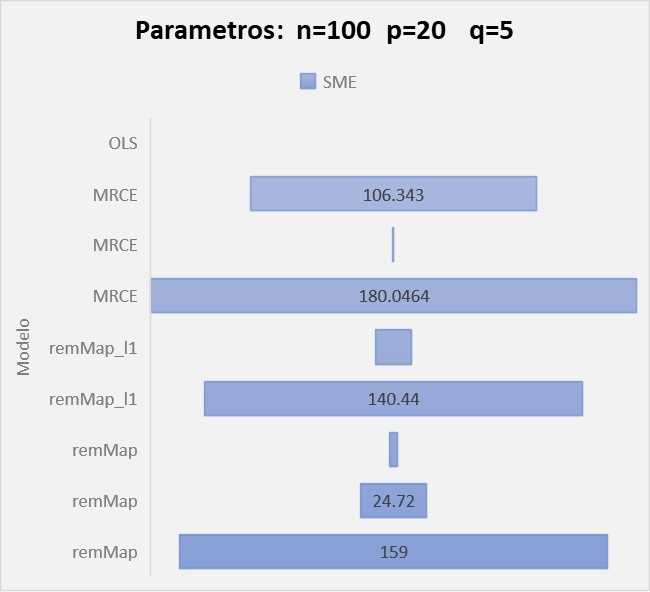
\includegraphics[scale=.65]{figure/im4.jpg}
  \caption{}
 \endminipage
\caption{MSE considerando distintos modelos, con $n>p$.}\label{R}
\end{figure}
Ahora, si consideramos cuando $n<p$ (ver Figura \ref{MSE_1}) notamos que los mejores predictores son ocupando algún método de regularización lo cual tienen sentido debido a que como existe más variables predictoras que registros se esta incumpliendo el supuesto de OLS y por ende los resultados no serían adecuados.

Es decir, pudimos observar el efecto que tiene utilizar los métodos de regularización cuando se incumple algún supuesto de mínimos cuadrados.
 \begin{figure}[H]
 \minipage{0.5\textwidth}
   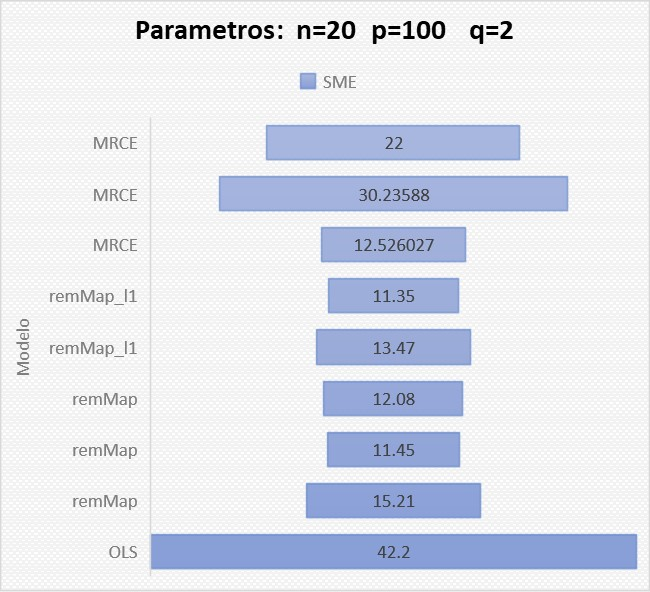
\includegraphics[scale=.65]{figure/im1.jpg}
  \caption{}
 \endminipage
 \minipage{0.5\textwidth}
   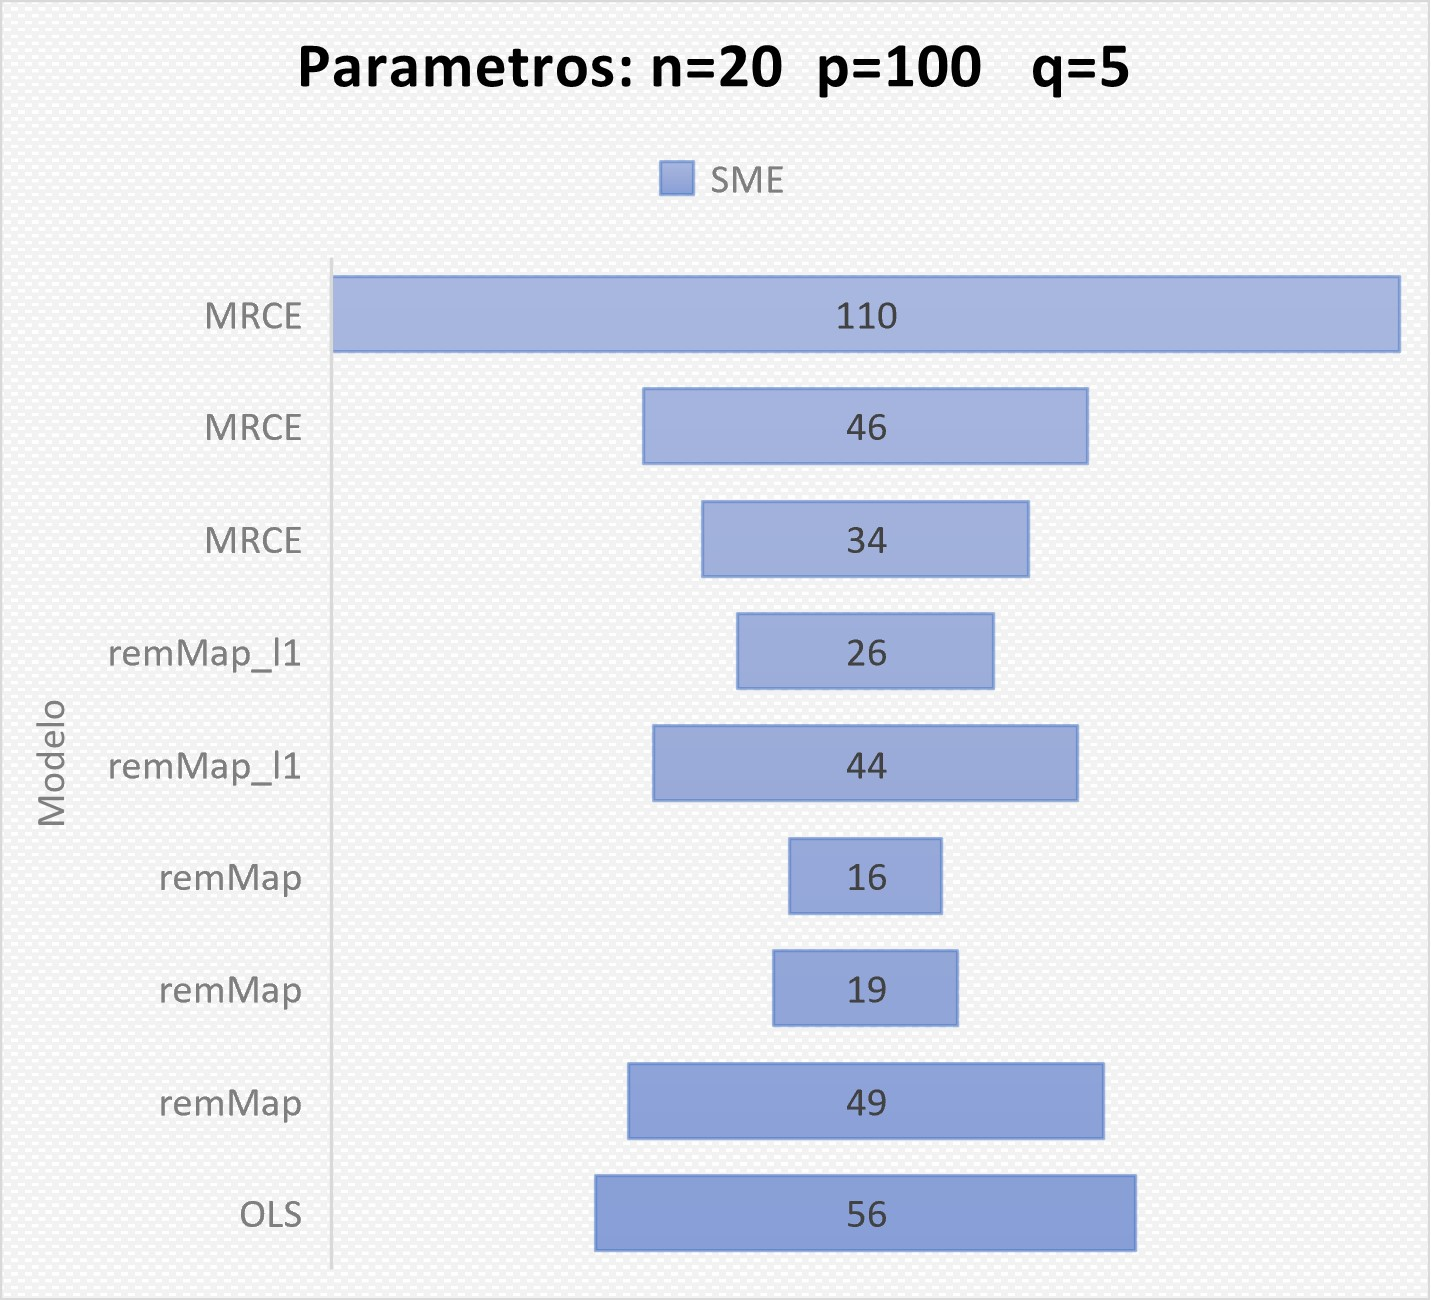
\includegraphics[scale=.65]{figure/im2.jpg}
  \caption{}
 \endminipage
 \caption{MSE considerando distintos modelos, con $n<p.$}\label{MSE_1}
 \end{figure}


\section{Conclusiones}
Se presentaron de forma concreta los principales métodos de regularización (\textit{ridge, LASSO y elastic net}) en regresión lineal multiple , y la importancia que tienen en comparación del enfoque clásico de mínimos cuadrados. Además, estos enfoques se pueden extender fácilmente a otro tipo de modelos: modelos lineales generalizados (regresión logística o poisson), modelos de supervicencia, etc.

Resaltamos que la regularización \textit{ridge} presenta mejores resultados cuando existe multicolinealidad en los datos esto se observa claramente en el ejemplo de \textit{contenido de grasa}, en donde la mayoría de las variables estaba correlaciones. Por otro lado, la regularización \textit{LASSO} presenta mejores resultados cuando se presenta un grupo de variables relevantes, y por consecuente es muy útil para poder interpretar los modelos ya que podemos este método restringe a los coeficientes a cero. Además, de que este método es ampliamente utilizada en \textit{feature selection} para un modelo de aprendizaje aútomatico más complejo. Y por último, la principal ventaja de la penalización de la red elástica es que permite una regularización eficaz a través de la penalización de \textit{ridge} con las características de selección de características de la penalización del \textit{LASSO}. Debido a que los métodos de regularización son aplicados a el tamaño del coeficiente, es de suma importancia estandarizar los datos antes de aplicar un método de regularización, esto se observo en el ejemplo de \textit{contenido de grasa} expuesto.


Además, desarrollamos la extensión de regularización para un modelo de regresión multivariada. En este caso presentamos el efecto que tiene los métodos de regularización cuando se incumple el supuesto de que existe un número de variables predictoras que número de registros, lo cuál es muy común en problemas de genoma o medicina.   

Es claro que este tipo de enfoque es muy importante no solo en métodos de regresión, si no en otros modelos. Ya que además de que es una alternativa cuando se violan cierto tipos de supuestos, también sirve como métodos para evitar \textit{overfitting} en problemas de aprendizaje automático. 

\section{Anexos}
\subsection{Códigos}
Todos las implementaciones se realizaron en el lenguaje de programación Python, en el sistema x86$\_$64, Ubuntu. Todos los códigos utilizados para estos resultados se pueden encontrar en mi página personal de Git-
gub: Enriquesec. En el repositorio Ciencia de Datos/Tareas/Proyecto$\_$final/. 

\subsection{Pseudo-algoritmos}
Aquí se presentan los pseudo-algoritmos de las metodologías propuestas de REMMAP y MCRE, en la sección \ref{multivariado}.

\begin{algorithm}[H]
\label{REMMAP_al}
 \KwIn{$Y_{n \times q}$,$X_{n \times p}$}
 \KwResult{$B_{p\times q}$}
Inicializamos parámetros, $[B=0_{p\times q},...]$;

\While{True}{
Para j=1,...p ; k=1,...,q
$$B_{j_0,k}=(|\X_{j_{0}}^{T} \tilde{\Y}_{k}|-\lambda_1)_{+} \frac{sign(\X_{j_{0}}^{T} \tilde{\Y}_{k})}{||\X_{j{0}}||_{2}^{2}} $$

\If{ ${B} $ no cambia }{
    \textbf{break}\;
    return(B)\;
}
}
\caption{ REMMAP \citep{remap}}
\end{algorithm}

\begin{algorithm}[H]
 \KwIn{$\Y_{n \times q}$,$\X_{n \times p}, \Omega_{p\times p}, \lambda_2$ y $\epsilon$}
 \KwResult{$\hat{B}_{p\times q}$}
$S=\X^T\X$\\
$H=\X^T\Y\Omega$\\
$\hat{\B}^{rigde}=(\X^T\X+\lambda_2I)^{-1}\X^T\Y.$\\

\While{$\sum|\hat{\B}^{(m)}-\hat{\B}^{m-1}|>\epsilon \sum|\hat{\B}^{rigde}|$}{

\For{r=1,...p}{
    \For{c=1,...,q}{
    $\mu_{rc}=\sum_{j=1}^p\sum_{k=1}^q \hat{b}_{jk}^{(m)}s_{rj}w_{kc}$\\
    $\hat{b}_{rc}^{(m)} = sign\left(\hat{b}_{rc}^{(m)}+\frac{h_{rc}-\mu_{rc}}{s_{rr}\omega_{cc}} \right) \left(\left| \hat{b}_{rc}^{(m)}+\frac{h_{rc}-\mu_{rc}}{s_{rr}\omega_{cc}} \right|-\frac{n\lambda_2}{s_{rr}\omega_{cc}}\right)_+$
    }
}
}
return$\left(\hat{\B}^{(m)}\right)$
 
\caption{Descenso de coordenadas cíclicas \citep{mrce}.} \label{algoritmo_1}
\end{algorithm}

\begin{algorithm}[H]
 \KwIn{$\Y_{n \times q}$,$\X_{n \times p}, \lambda_1, \ \lambda_2, \epsilon.$}
 \KwResult{$\hat{B}_{p\times q}$}
 \textit{Inicializamos}\\
 $\hat{\B}^{(0)}=0$\\
 $\hat{\Omega}^{(0)}=\hat{\Omega}(\hat{\B}_^{(0)})$\\

\While{$\sum|\hat{\B}^{(m)}-\hat{\B}^{m-1}|>\epsilon \sum|\hat{\B}^{rigde}|$}{

    \begin{enumerate}
        \item Calcular $\hat{\B}^{m+1}=\hat{\B}(\hat{\Omega}^{(m)}$ resolviendo \ref{est_beta} utilizando el \textbf{Algoritmo \ref{algoritmo_1}}.
        \item Calcular $\hat{\Omega}^{(m+1)}=\hat{\Omega}(\hat{\B}^{(m+1)})$ resolviendo \ref{cov_estimate} usando el algoritmo de LASSO gráfico.
    \end{enumerate}

}
return$\left(\hat{\B}^{(m)}\right)$
 
\caption{MRCE \citep{mrce}.} \label{algoritmo_2}
\end{algorithm}


\subsection{Algoritmo de LASSO gráfico}
\cite{friedman_sparse_2008} describe este método para máximizar el problema de optimización \textbf{(\ref{cov_estimate})}. Sea $W$ el estimador para $\Sigma$ (matriz de covarianza poblacional). Se puede mostrar que se puede resolver el problema optimizando cada fila y la columna correspondiente a $W$ en una forma de descenso de coordenadas de bloque. Partimos $W$ y $S$,
\begin{align*}
    W=\begin{pmatrix}
    W_{11} & w_{12}\\
    w_{12}^T & w_{22}
    \end{pmatrix}, \ \ \ S= W=\begin{pmatrix}
    S_{11} & s_{12}\\
    s_{12}^T & s_{22}
    \end{pmatrix}
\end{align*}
donde $S$ es la matriz de correlación empírica. Entonces se puede mostrar que
\begin{align}\label{ww}
    w_{12}=\arg \min_y\left\{y^TW_{11}^{-1}y:||y-s12||_\infty\geq p \right\}.
\end{align}
Lo anterior es un programa cuadrático con restricciones de caja que resuelven usando un procedimiento de punto interior. Pero de igual manera se puede mostrar usando dualidad convexa que el problema (\ref{ww}) es  equivalente a resolver el problema dual
\begin{align}\label{www}
    \min_\beta \left\{\frac{1}{2} |W_{11}^{-1/2}\beta-b|^2+\lambda|\beta|_1 \right\}
\end{align}
donde $b=W_{11}^{-1/2}s_{12}$. Si $\beta$ resuelve (\ref{www}) entonces $w_{12}=W_{11}\beta$ resuelve (\ref{ww}). Además es sencillo ver que las soluciones en (\ref{cov_estimate}) son equivalentes a resolver (\ref{www}). Para resolver (\ref{www}) usamos $W_{11}$ y $s$. Luego actualizamos $w$ y corremos todas las variables hasta la convergencia. Consideramos que la solución de $w_{ii}=s_{ii}+\lambda$ para todo $i$. Este algoritmo se le conoce como algoritmo \textit{LASSO} gráfico (ver \textbf{Algoritmo} \ref{algoritmo_lasso}).

\begin{algorithm}[H]
 \KwIn{$S, \lambda$ y $\epsilon$.}
 \KwResult{$W$}
 \textit{Inicializamos}\\
 $W=S+\lambda\rho$

\While{$|W-\{diagonal\}|>\epsilon |S-\{diagonal\}|$}{
    \For{j=1,2,\cdots, p, 1,2, \cdots, p, \cdots}{
    Resolver el problema de LASSO en (\ref{www}). Esto regresa un vector solución $\hat{\beta}$ de tamaño $p-1$, por lo que imputamos el renglón y la columna de $W$ usando $w_{12}=W_{11}\hat{\beta}.$
    }
}
return$\left(W^{-1}\right)$
 
\caption{LASSO gráfico \citep{friedman_sparse_2008}} \label{algoritmo_lasso}
\end{algorithm}

Para resolver el paso 5 del (\textbf{Algoritmo} \ref{algoritmo_lasso}) consideramos un descenso coordinado. Sea $V=W_{11}$ y $u=s_{12},$ entonces actualizamos $\beta_j$ de la forma
\begin{align}
    \hat{\beta}_j = S(u_j- \sum_{k\neq j} V_{jk}\beta_k, \lambda) /V_{jj}
\end{align}
para $j=1,2,\cdots, p, 1,2, \cdots, p, \cdots.$ Donde $S$ es el operador soft-threshold:
$$S(x,y)=sign (x)(|x|-t)_+.$$
Para más detalle de este algoritmo consulte \cite{friedman_sparse_2008}, ahí se presentan las demostraciones más a detalle y más referencias sobre problemas similares. 

\subsection{Descenso de coordenadas cíclicas}
\label{descenso_coo}
El descenso de coordenadas es un algoritmo de optimización que minimiza sucesivamente a lo largo de las direcciones de las coordenadas para encontrar el mínimo de una función. En nuestro problema, tenemos la función objetivo para $\Omega$ fija en $\Omega_0$ es
\begin{align}
    f(\B)=g(\B,\Omega)+\lambda_2+\sum_{j=1}^p\sum_{k=1}^q |b_{jk}|
\end{align}
Se puede resolver para $\B$ utilizando un descenso de coordenadas cíclicas. Expresamos las derivadas direccionales como
\begin{align}
    \frac{\partial f+}{\partial\B} = \frac{2}{n}\X^T\X\B\Omega-\frac{2}{n}\X^T\Y\Omega+\lambda_21_{(b_{ij}>0)}-\lambda_21_{(b_{ij}<0)}\\
    \frac{\partial f-}{\partial\B} = -\frac{2}{n}\X^T\X\B\Omega+\frac{2}{n}\X^T\Y\Omega-\lambda_21_{(b_{ij}>0)}+\lambda_21_{(b_{ij}<0)}
\end{align}
donde $1_{(.)}$ es un indicador. Si definimos a $S=\X^T\X$ y $H=\X^T\Y\Omega$ y $\mu_{rc}=\sum_{j=1}^p\sum_{k=1}^q b_{jk}s_{rj}w_{kc}$, entonces considerando un solo parametro $b_{rc}$ tenemos que las derivadas direccionales son
\begin{align*}
    \frac{\partial f+}{\partial b_{rc}} = \mu_{rc}-h_{rc}+n\lambda_21_{(b_{ij}>0)}-n\lambda_21_{(b_{ij})<0},\\
     \frac{\partial f-}{\partial b_{rc}} = -\mu_{rc}+h_{rc}-n\lambda_21_{(b_{ij}>0)}+n\lambda_21_{(b_{ij})<0}.
\end{align*}
Sea $b_{rc}^0$ nuestra iteración actual, entonces míminizar lo anterior es equivalente a resolver $\hat{b}_{rc}^*$
\begin{align*}
    \hat{b}_{rc}^*s_{rr}\omega_{cc}-b^0_{rc}s_{rr}\omega_{cc}+\mu_{rc}-h_{rc}=0.
\end{align*}

Por lo anterior, es sencillo ver que implica que 
\begin{align*}
    \hat{b}_{rc}=sign\left( \hat{b}^*_{rc}\right)\left(\left| \hat{b}^*_{rc}\right|-\frac{n\lambda_2}{s_{rr}\omega_{cc}} \right)_+.
\end{align*}
Si $\hat{b}^*_{rc}=0$ tiene un valor de cero, entonces tanto la parte de pérdida como la de penalización de la función objetivo se minimizan y el párametro permance en 0. Por lo que podemos escribir esta solución como
\begin{align*}
    \hat{b}_{rc}=sign\left( \hat{b}^0_{rc}+\frac{h_{rc}-\mu_{rc}}{s_{rr}\omega_{cc}}\right)\left(\left| \hat{b}^0_{rc}+\frac{h_{rc}-\mu_{rc}}{s_{rr}\omega_{cc}}\right|-\frac{n\lambda_2}{s_{rr}\omega_{cc}} \right)_+.
\end{align*}

\newpage

\bibliographystyle{unsrtnat}
\bibliography{biblio}  %%% Uncomment this line and comment out the ``thebibliography'' section below to use the external .bib file (using bibtex) .



\end{document}